% \pagebreak[4]
% \hspace*{1cm}
% \pagebreak[4]
% \hspace*{1cm}
% \pagebreak[4]
%\usepackage[round,colon,authoryear]{natbib}

\chapter{A pipeline for the analysis of TraDIS experiments, with an application to {\it Salmonella} macrophage invasion}
\label{sec:chapterPingpong}
\ifpdf
    \graphicspath{{Chapter3/Chapter3Figs/EPS/}{Chapter3/Chapter3Figs/}}
\fi

\textit{Section 3.3 describes a collaborative study with Gemma C. Langridge (Pathogen Genomics, Wellcome Trust Sanger Institute). Gemma performed all laboratory experiments described in this chapter.}

\section{Introduction}

In the previous chapter, I described the results of a study predicting and comparing the genes required for robust growth of two \textit{Salmonella} serovars in standard laboratory media. While this revealed interesting aspects of \textit{Salmonella} biology, linking these findings to \textit{Salmonella}'s infective niche in the human host is difficult. However, transposon-insertion sequencing can be used to interrogate infective conditions directly (reviewed previously in section 1.5): by comparing libraries passed through a condition of interest to control libraries, we can determine the genomic regions involved in survival in that condition. In this chapter, I describe a pipeline for the analysis of such experiments, illustrated with an experiment assaying genes required for \textit{S.} Typhi and Typhimurium invasion of (or uptake into) human macrophage.

\subsection{\textit{Salmonella} interactions with macrophage}

As previously described in section 2.1, the ability to invade and survive in host cells was a major factor in the early evolution of \textit{S. enterica} subspecies \textit{enterica}. This appears to have been largely driven by the acquisition of two horizontally-acquired pathogenicity islands, SPI-1 and -2. Due to the availability of a mouse model\parencite{Santos2001}, most of what is known about \textit{Salmonella} interactions with host cells is derived from studies of \textit{S.} Typhimurium infection. 

\textit{S.} Typhimurium infections of either epithelial or phagocytic cells appear to follow broadly similar paths (\textcite{Figueira2012}, see also figure \ref{fig:SCV}). The SPI-1 T3SS is induced, and  

\begin{figure}[htp]
\begin{center}
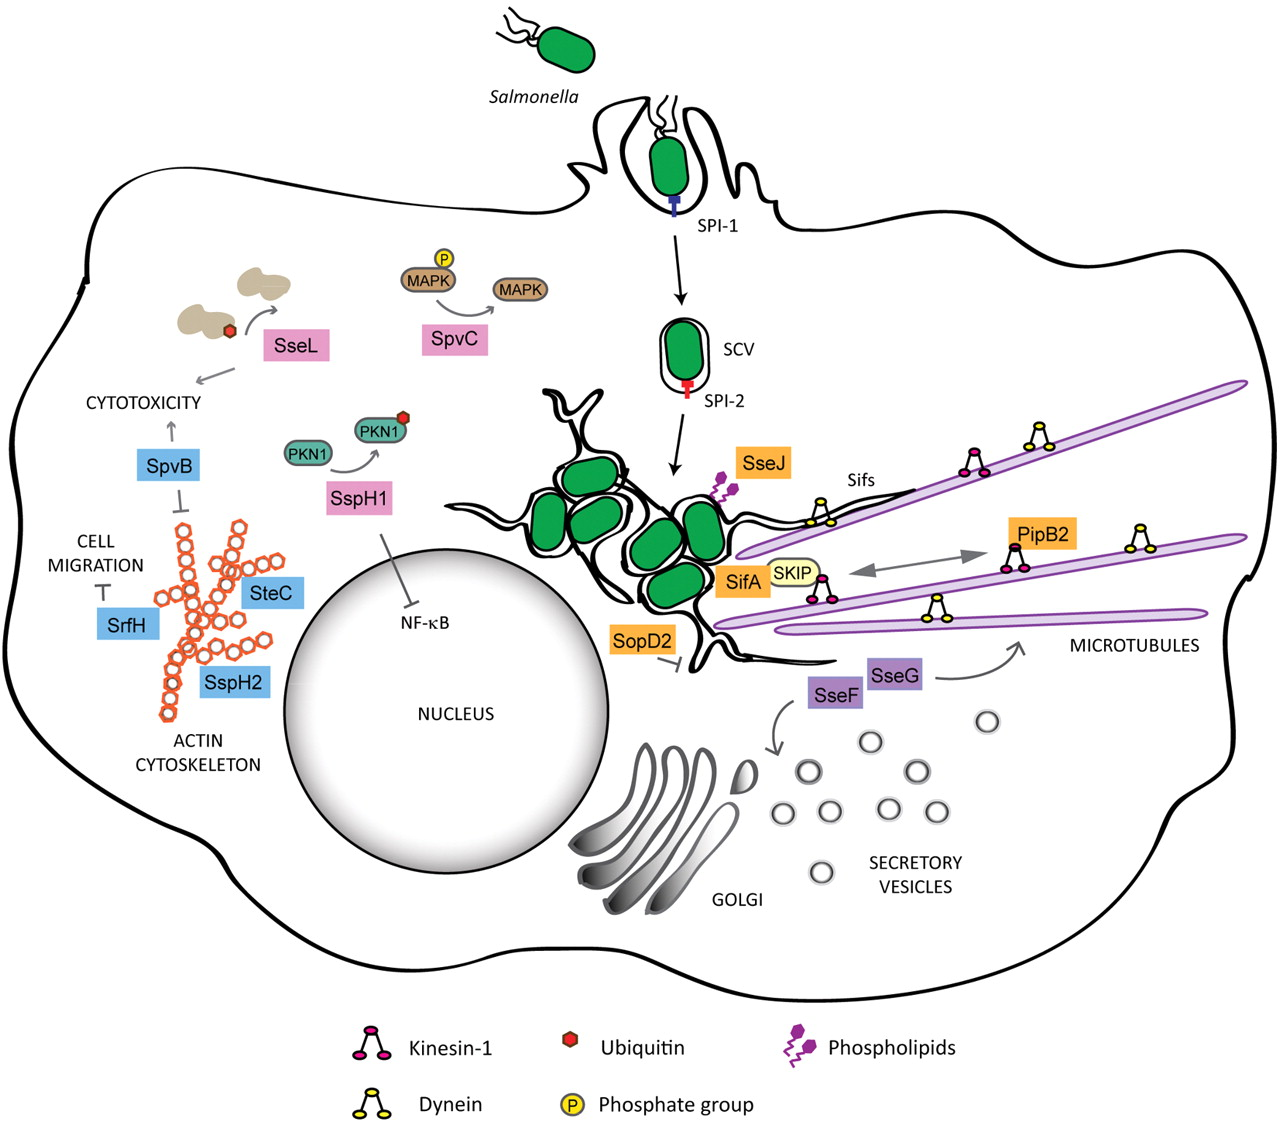
\includegraphics[width=14cm]{SCV.jpg}
\caption[Biogenesis of the \textit{Samonella} containing vacuole]{\textbf{Biogenesis of the \textit{Samonella} containing vacuole (SCV).} \textit{Salmonella} adheres to the outer membrane of host cells, and uses SPI-1 and its associated effectors to induce membrane ruffling and entry into the SCV. The SPI-2 T3SS functions mainly in maintenance of the SCV, through the action of the effectors SifA, SopD2, SseJ and PipB2 (orange boxes), and its localization near the Golgi of host cells, mediated by SseF and SseG (purple boxes). Other effectors are involved in modulation of host immune signalling (SpvC, SspH1 and SseL; pink boxes) or target the host cytoskeleton (SteC, SpvB, SspH2 and SrfH; blue boxes). Reproduced from \textcite{Figueira2012} under a Creative Commons Attribution License (CCAL). 
} 
\label{fig:SCV}
\end{center}
\end{figure}

\section{Methods}

Determining conditional gene fitness presents a somewhat different problem to that addressed in the previous chapter, predicting and comparing ``essential'' genes under the conditions of library creation. In predicting gene essentiality, we had a single time point representing the initial growth of the library on rich media, while in identifying conditional gene fitness (measured as the relative expansion or contraction of mutant populations) we are always comparing changes in mutant fitness with respect to fitness in a baseline condition. In some ways, this makes the problem of identifying genes with strong fitness effects easier: as we are primarily interested in the ratio of various insertion mutants present between the two conditions, effects that may confound the prediction of simple gene essentiality are effectively ``zeroed out''. More explicitly, whether low insertion density in the library occurs due to chance, nucleotide composition bias, or the exclusionary effects of high-density DNA-binding proteins (described in section 2.3.3) does not matter -- these regions can simply be identified as not producing sufficient reads over insertion-sites to be assayed and removed from the analysis.

In many ways, the problem of investigating the statistical and biological significance of ratios of reads over insertion sites resembles established analyses developed for differential RNA-seq analysis. In this section I describe the

\subsection{Mapping insertion sites}

\subsection{Defining genomic features}

\subsection{Quality control}

\subsection{Inter-library normalization}

\subsection{Identifying fitness effects}

\subsection{Functional analysis of gene sets that affect fitness}

\section{Application: \textit{Salmonella enterica} macrophage invasion}

\subsection{Background: the {\it Salmonella} containing vacuole}

\subsection{Experimental methods}

\textit{All experiments were performed by Gemma Langridge. They are described here briefly for completeness; in-depth descriptions of the experiments are available in \parencite{Langridge2010}}


\subsection{Results}

\subsection{Other applications}